\exercisesection{COHEN 环}

在 § 2 的习题中，\(p\) 是一个固定的素数。若 \(a\) 是环 A 的理想，则用 \(a^p\) 表示由元素 \(a^p\)（其中 \(a\) 取遍 \(a\)）所生成的理想。

\begin{enumerate}
\def\labelenumi{\arabic{enumi})}
\item
  设 \((\mathbf{C}_{n}, \pi_{n,m})\) 是关于指标集 N 的环的逆系统。假设 \(C_{n}\)（对每个 \(n \in N\)）都是 Artin 环，且诸同态 \(\pi_{n,m}\) 都是满射。设 \(\pi_{n}\) 是从 \(C = \varprojlim C_{n}\) 到 \(C_{n}\) 的典范同态。证明对所有 \(x \in C\)，有 \(xC = \varprojlim \pi_{n}(x) C_{n}\)。（按 § 2, n° 1 命题 3 的证明方式处理。）
\item
  设 A 是环，\((\mathbf{J}_{n})_{n\in\mathbb{N}}\) 是 A 的理想的一个递降序列，使得有 \(pJ_{n} + J_{n}^{p} \subset J_{n+1}\)（对每个 \(n \in N\)）。
\end{enumerate}

\begin{enumerate}
\def\labelenumi{\alph{enumi})}
\item
  证明在这一假设下，§ 1, n° 1 的引理 1 与命题 1 的断言仍然成立。
\item
  设 \(i\) 与 \(n\) 是两个正整数。当 \(i \leqslant n\) 时，从 A 到 A 的映射 \(x \mapsto p^i x^{p^n - i}\) 通过过渡到商定义了一个映射
\end{enumerate}

\[
\rho_ {n, i} ^ {\mathbf {A}}: \mathrm{A} / \mathrm{J} _ {0} \rightarrow \mathrm{A} / \mathrm{J} _ {n}.
\]

当 \(i > n\) 时，令 \(\rho_{n,i}^{\mathbf{A}} = 0\)。对 \(x \in \mathrm{A} / \mathrm{J}_n\) 与 \(a \in \mathrm{A} / \mathrm{J}_0\)，有 \(x^{p^{n - i}} \rho_{n,i}^{\mathbf{A}}(a) = \rho_{n,i}^{\mathbf{A}}(\overline{x} a)\)，其中 \(\overline{x}\) 是 \(x\) 在 \(\mathrm{A} / \mathrm{J}_0\) 中的像。若 \(j\) 是正整数，且 \(a, b\) 是 \(\mathrm{A} / \mathrm{J}_n\) 的两个元素，则有

\[
\rho_ {n, i} ^ {\mathbf {A}} (a) \rho_ {n, j} ^ {\mathbf {A}} (b) = \rho_ {n, i + j} ^ {\mathbf {A}} \left(a ^ {p ^ {j}} b ^ {p ^ {i}}\right).
\]

\begin{enumerate}
\def\labelenumi{\alph{enumi})}
\setcounter{enumi}{2}
\tightlist
\item
  设 \((\mathbf{R}_{n})_{n\in\mathbf{N}}\) 是第 42 页习题 3 中构造的多项式序列。设 n 与 i 是两个正整数，a 与 b 是 \(A/J_{0}\) 的两个元素。于是在 \(A/J_{n}\) 中有等式
\end{enumerate}

\[
\rho_ {n, i} ^ {\mathrm{A}} (a) + \rho_ {n, i} ^ {\mathrm{A}} (b) = \sum_ {m = 0} ^ {n - i} \rho_ {n, i + m} ^ {\mathrm{A}} (\mathrm{R} _ {m} (a, b)).
\]

\begin{enumerate}
\def\labelenumi{\arabic{enumi})}
\setcounter{enumi}{2}
\tightlist
\item
  设 \(n\) 是正整数。设 C 是 \(p\)-Cohen 环，其剩余域为 \(k\)，长度为 \(n+1\)。设 \((x_{\lambda})_{\lambda\in\Lambda}\) 是 C 中提升 \(p\)-基 \((\xi_{\lambda})_{\lambda\in\Lambda}\)（\(k\) 的）的元素族。用 \(\rho_{i}:k\to C\)（对每个 \(i\in\mathbf{N}\)）表示习题 2 中定义的映射 \(\rho_{n,i}^{\mathrm{C}}\)，其中 \(\mathbf{J}_{m}\) 取理想 \(p^{m+1}\mathbf{C}\)。
\end{enumerate}

\begin{enumerate}
\def\labelenumi{\alph{enumi})}
\tightlist
\item
  对 \(r \in \mathbf{N}\)，用 \(\mathbf{M}_r\) 表示由重指标 \(m \in \mathbf{N}^{(\Lambda)}\)（满足对每个 \(\lambda \in \Lambda\) 有 \(0 \leqslant m_{\lambda} < p^{r}\)）所成的集合。于是，对 C 的每个元素 \(\alpha\)，存在唯一的有限支撑族 \((a_{i,m})\)（\(0 \leqslant i \leqslant n\)，\(m \in \mathbf{M}_{n-i}\)），其元素属于 \(k\)，使得
\end{enumerate}

\[
\alpha = \sum_ {i = 0} ^ {n} \sum_ {m \in \mathbf {M} _ {n - i}} \rho_ {i} (a _ {i, m}) x ^ {m},
\]

其中记号 \(x^{m}\) 表示乘积 \(\prod x_{\lambda}^{m_{\lambda}}\)。

\begin{enumerate}
\def\labelenumi{\alph{enumi})}
\setcounter{enumi}{1}
\tightlist
\item
  考虑由生成元 \([x_{\lambda}]\)（\(\lambda\) 取遍 \(\Lambda\)）与 \([\rho_{i}(a)]\)（i 取遍 N，a 取遍 k）所生成的环 U，这些生成元只须满足下列关系（其中多项式 \(R_{i}\) 是第 42 页习题 3 中引入的那些）。
\end{enumerate}

\begin{enumerate}
\def\labelenumi{(\roman{enumi})}
\item
  \([\rho_i(a)] = 0\) 对 \(a \in k, i > n\) 成立，
\item
  \(\left[\rho_0(1)\right] = 1\) 且 \(\left[\rho_0(0)\right] = 0,\)
\item
  \([\rho_i(a)][\rho_j(b)] = [\rho_{i + j}(a^{p^j}b^{p^i})]\) 对 \(i,j\)（属于 \(\mathbf{N}\)）与 \(a,b\)（属于 \(k\)）成立，
\item
  \([\rho_i(a)] + [\rho_i(b)] = \sum [\rho_{i+m}(\mathbf{R}_m(a,b))]\)（对 \(i\in \mathbf{N}\) 与 \(a,b\)（属于 \(k,\)）），
\item
  \([x_{\lambda}]^{p^{n - i}}[\rho_i(a)] = [\rho_i(\xi_{\lambda}a)]\) 对 \(0 \leqslant i \leqslant n, \lambda \in \Lambda, a \in k\) 成立。
\end{enumerate}

证明我们有 \([\rho_i(0)] = 0\)（对每个 \(i \in \mathbf{N}\)）。

利用第 42 页习题 3 b) 证明：若 \(p\) 为奇数，则有 \([\rho_0(-1)] = -1\)；若 \(p\) 为偶数，则有 \(\sum_{i=0}^{n} [\rho_i(1)] = -1\)。

\begin{enumerate}
\def\labelenumi{\alph{enumi})}
\setcounter{enumi}{2}
\tightlist
\item
  存在唯一的从 U 到 C 的映射，它把 U 中与每个有限支撑族 \((a_{i,m})_{0\leqslant i\leqslant n,m\in M_{n - i}}\)（其元素属于 \(k\)）相伴的元素
\end{enumerate}

\[
\left\langle \left(a _ {i, m}\right) \right\rangle = \sum_ {i = 0} ^ {n} \sum_ {m \in \mathbf {M} _ {n - i}} \left[ \rho_ {i} (a _ {i, m}) \right] \prod_ {\lambda \in \Lambda} [ x _ {\lambda} ] ^ {m _ {\lambda}}
\]

映到 C 的元素 \(\sum_{i=0}^{n}\sum_{m\in M_{n-i}}\rho_i(a_{i,m})x^m\)；它是环同构。

\begin{enumerate}
\def\labelenumi{\alph{enumi})}
\setcounter{enumi}{3}
\tightlist
\item
  由前述结果给出 § 2, n° 3 各结果的另一个证明。
\end{enumerate}

\begin{enumerate}
\def\labelenumi{\arabic{enumi})}
\setcounter{enumi}{3}
\tightlist
\item
  设 C 是无限长度的 \(p\)-Cohen 环，\(k\) 是其剩余域。设 A 是环，\((\mathbf{J}_n)_{n \in \mathbb{N}}\) 是 A 的理想的递降序列，满足 \(p\mathbf{J}_n + \mathbf{J}_n^p \subset \mathbf{J}_{n+1}\)（对每个 \(n \in \mathbb{N}\)）。最后，设 \(\overline{\varphi}: k \to \mathrm{A} / \mathrm{J}_0\) 是环同态，\((\xi_\lambda)_{\lambda \in \Lambda}\) 是一个 \(p\)-基（\(k\) 的），\((x_\lambda)_{\lambda \in \Lambda}\) 是 C 中提升该 \(p\)-基的元素族，而 \((a_\lambda)_{\lambda \in \Lambda}\) 是 A 中元素的族，使得 \(a_\lambda\) 在 \(\mathrm{A} / \mathrm{J}_0\) 中的像为 \(\overline{\varphi}(\xi_\lambda)\)。
\end{enumerate}

\begin{enumerate}
\def\labelenumi{\alph{enumi})}
\item
  对每个 \(n\in\mathbf{N}\)，存在唯一的同态 \(\varphi_{n}\)（从 \(\mathrm{C}/p^{n+1}\mathrm{C}\) 到 \(\mathrm{A}/\mathrm{J}_{n}\)），使得 \(\varphi_{n}\circ\rho_{n,i}^{\mathrm{C}}=\rho_{n,i}^{\mathrm{A}}\circ\overline{\varphi}\)，且使得 \(\varphi_{n}\) 把 \(x_{\lambda}\) 的类映为 \(a_{\lambda}\) 的类。（利用习题 2 与习题 3。）
\item
  假设 A 对滤过 \((\mathrm{J}_{n})_{n\in\mathbb{N}}\) 所定义的拓扑是分离的且完备的。则存在唯一的从 C 到 A 的环同态 \(\varphi\)，使得 \(\varphi(x_{\lambda}) = a_{\lambda}\)（对 \(\lambda \in \Lambda\)），且 \(\varphi\) 通过过渡到商诱导 \(\overline{\varphi}\)。这一同态是连续的。
\item
  假设环 A 是局部的、分离的且完备的，有 \(J_{n} = m_{A}^{n+1}\)（对每个 \(n \in N\)），有 \(A/J_{0} = k\)，且 \(\overline{\varphi}\) 是恒等映射。证明在 \(\varphi\) 之下 C 在 A 中的像是 \(A'\) 的包含每个元素 \(a_{\lambda}\) 的唯一 Cohen 子环，从而给出 § 2, n° 2 定理 1 的 a) 款的另一个证明；若 k 是完美的且 C 是环 W(k)，则得到 § 2, n° 4 定理 2 的另一个证明。
\end{enumerate}

\begin{enumerate}
\def\labelenumi{\arabic{enumi})}
\setcounter{enumi}{4}
\tightlist
\item
  设 A 是环，\((\mathrm{J}_n)_{n\in \mathbb{N}}\) 是 A 的理想的递降序列，满足 \(p\mathbf{J}_n + \mathbf{J}_n^p\subset \mathbf{J}_{n + 1}\)（对每个整数 \(n\geqslant 0\)）。设 R 是特征为 \(p\) 的环，\(\overline{\varphi}\) 是从 R 到 \(\mathrm{A} / \mathrm{J}_0\) 的环同态。称 \(\overline{\varphi}\) 到 \(\mathrm{A} / \mathrm{J}_n\) 中的一个提升为一个映射 \(\varphi_n:\mathbb{R}\to \mathbb{A} / \mathbb{J}_n\)，它满足 \(\varphi_n(x^p) = \varphi_n(x)^p\)（对 \(x\in \mathbb{R}\)），且通过过渡到商重新给出 \(\overline{\varphi}\)。a) 设 \(\varphi_n\) 与 \(\widetilde{\varphi}_n\) 是 \(\overline{\varphi}\) 在 \(\mathrm{A} / \mathrm{J}_n\) 中的两个提升。则 \(\varphi_n\) 与 \(\widetilde{\varphi}_n\) 在 \(\mathbb{R}^{p^n}\) 上一致。b) 若 R 是完美的，则存在 \(\varphi_n\)（\(\overline{\varphi}\) 在 \(\mathrm{A} / \mathrm{J}_n\) 中的唯一提升）。我们有 \(\varphi_n(1) = 1\)，且有 \(\varphi_n(xy) = \varphi_n(x)\varphi_n(y)\)（对 \(x,y\in \mathbb{R}\)）。
\end{enumerate}

\begin{enumerate}
\def\labelenumi{\arabic{enumi})}
\setcounter{enumi}{5}
\tightlist
\item
  设 A 是环，\((\mathbf{J}_{n})_{n\in\mathbb{N}}\) 是 A 的理想的递降序列。假设 A 对滤过 \((\mathbf{J}_{n})_{n\in\mathbb{N}}\) 所定义的拓扑是分离的且完备的，且有 \(pJ_{n} + J_{n}^{p} \subset J_{n+1}\)（对每个整数 \(n \geqslant 0\)）。用 \(\pi_{n}\) 表示从 A 到 \(A/J_{n}\) 上的典范映射。设 R 是特征为 p 的完美环，\(\overline{\varphi}\) 是从 R 到 \(A/J_{0}\) 的环同态。
\end{enumerate}

\begin{enumerate}
\def\labelenumi{\alph{enumi})}
\item
  存在唯一的从 R 到 A 的映射 \(\varphi\)，使得有 \(\overline{\varphi} = \pi_0 \circ \varphi\)，且 \(\varphi(x^p) = \varphi(x)^p\)（对每个 \(x \in \mathbb{R}\)）。此外，我们有 \(\varphi(1) = 1\) 与 \(\varphi(xy) = \varphi(x)\varphi(y)\)（对 R 中的 \(x\) 与 \(y\)）。当 A 是特征为 \(p\) 的环时，\(\varphi\) 是环同态。（可利用前一习题。）
\item
  对每个 \(n\in\mathbf{N}\)，存在唯一的环同态 \(v_{n}:W_{n+1}(A/J_{0})\to A/J_{n}\)，它使下图成为交换的
\end{enumerate}

\pandocbounded{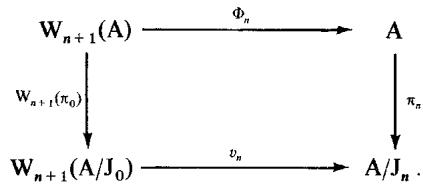
\includegraphics[keepaspectratio]{images/part002_309b7be5.jpg}}

\begin{enumerate}
\def\labelenumi{\alph{enumi})}
\setcounter{enumi}{2}
\tightlist
\item
  置 \(u_n = v_n \circ \mathbf{W}_{n+1}(\overline{\varphi}) \circ \mathbf{F}^{-n}\)。于是，对每个 \(n \in \mathbf{N}\)，下图（其中竖直箭头表示典范投影）是交换的
\end{enumerate}

\pandocbounded{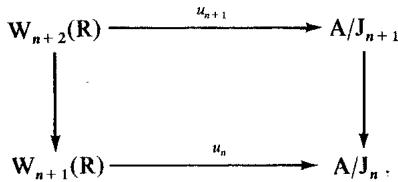
\includegraphics[keepaspectratio]{images/part002_feb0ecf4.jpg}}

\begin{enumerate}
\def\labelenumi{\alph{enumi})}
\setcounter{enumi}{3}
\tightlist
\item
  存在唯一的环同态 u，使下图成为交换的。
\end{enumerate}

\pandocbounded{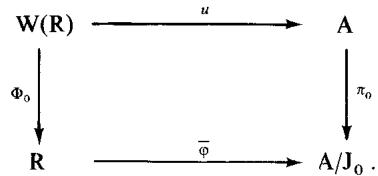
\includegraphics[keepaspectratio]{images/part002_890d1cac.jpg}}

  同态 \(u\) 是连续的（当 \(\mathbf{W}(\mathbf{R})\) 赋有 \(p\)-进拓扑时），且对每个 \(\boldsymbol{a} = (a_n)_{n \in \mathbb{N}} \in \mathbf{W}(\mathbf{R})\)，有 \(u(\boldsymbol{a}) = \sum_{n=0}^{\infty} p^n \varphi(a_n^{p^{-n}})\)。

（\(u\) 的存在性由前述可得。为证明 \(u\) 的唯一性、连续性及其显式表达式，利用等式 \(\varphi = u \circ \tau\)，其中 \(\varphi\) 是 a) 中构造的从 R 到 A 的映射，而 \(\tau: \mathrm{R} \to \mathrm{W(R)}\) 是 § 1, n° 5 中定义的映射。）

\begin{enumerate}
\def\labelenumi{\alph{enumi})}
\setcounter{enumi}{4}
\tightlist
\item
  给出 § 2, n° 4 定理 2 的另一个证明，它不同于正文中的证明，也不同于习题 4, c) 中的证明。
\end{enumerate}

\begin{enumerate}
\def\labelenumi{\arabic{enumi})}
\setcounter{enumi}{6}
\tightlist
\item
  \begin{enumerate}
  \def\labelenumii{\alph{enumii})}
  \tightlist
  \item
    设 R 是特征为 p 的完美环，R' 是特征为 p 的环。设 f 是从 R 到 R' 中的同态。则同态 W(f): W(R) → W(R') 是使下图成为交换的唯一同态。
  \end{enumerate}
\end{enumerate}

\pandocbounded{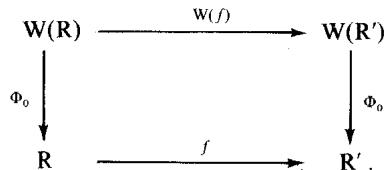
\includegraphics[keepaspectratio]{images/part002_f36acea2.jpg}}

（利用前一习题。）

特别地，取 \(f\) 为 R 上的 p 次幂映射，证明 \(\mathrm{F}_{\mathrm{R}}\) 是 \(\mathbf{W}(\mathbf{R})\) 的使得 \(\Phi_{0} \circ \mathrm{F}_{\mathrm{R}} = f \circ \Phi_{0}\) 的唯一自同态。它由等式

\[
\mathrm{F} _ {\mathbf {R}} (\tau (x)) = \tau (x ^ {p}) \quad \text { for all } \quad x \in \mathbf {R}  .
\]

\begin{enumerate}
\def\labelenumi{\alph{enumi})}
\setcounter{enumi}{1}
\tightlist
\item
  设 A 是对 p-进拓扑分离且完备的环。假设 A 中乘以 \(p.1_{A}\) 的乘法是单射，且 A/pA 是完美环。则存在唯一的 A 的自同态 \(\sigma\)，使得 \(\sigma(x) \equiv x^{p} \mod pA\)（对 \(x \in A\)），且第 44 页习题 14 中所述的同构 \(t_{\sigma}: A \to W(A/pA)\) 的逆由
\end{enumerate}

\[
(a _ {i}) _ {i \in \mathbf {N}} \mapsto \sum_ {i = 0} ^ {\infty} \varphi (a _ {i}) ^ {p ^ {- i}} p ^ {i},
\]

给出，其中 \(\varphi : \mathrm{A} / p\mathrm{A} \to \mathrm{A}\) 是通过过渡到商给出 \(\mathrm{A} / p\mathrm{A}\) 的恒等映射、且满足 \(\varphi(x^p) = \varphi(x)^p\)（对 \(x \in \mathbb{R}\)）的唯一映射（参见习题 6, a)）。

\begin{enumerate}
\def\labelenumi{\arabic{enumi})}
\setcounter{enumi}{7}
\item
  设 C 是以 k 为剩余域的无限长度 p-环。k 的每个自同构都可扩张为 C 的自同构。C 的通过过渡到商在 k 上诱导恒等映射的自同构是恒等映射，当且仅当 k 是完美的。
\item
  设 \(k\) 是特征为 \(p\) 的域，\(\mathbf{C}_k\) 是无限长度的 \(p\)-环（以 \(k\) 为剩余域）。设 A 是分离且完备的局部环，\(u: \mathbf{C}_k \to \mathbf{A}\) 是局部同态，使得由 \(u\) 通过过渡到商得到的同态使 A 的剩余域 K 成为 \(k\) 的可分扩张。设 \(\mathbf{C}_{\mathbf{K}}\) 是以 K 为剩余域的无限长度 \(p\)-环。证明存在局部同态 \(i: \mathbf{C}_k \to \mathbf{C}_{\mathbf{K}}\) 与 \(v: \mathbf{C}_{\mathbf{K}} \to \mathbf{A}\)，使得 \(u = v \circ i\)，且 \(v\) 通过过渡到商在 K 上诱导恒等映射。
\item
  设 \(k\) 是特征为 \(p\) 的域，\((\xi_{\lambda})_{\lambda \in \Lambda}\) 是一个 \(p\)-基（\(k\) 的），且对每个整数 \(n \geqslant 1\)，用 \(C_n\) 表示 \(\mathbf{W}_n(k)\) 的由 \(\mathbf{W}_n(k^{p^{n-1}})\) 与诸元素 \(\tau(\xi_{\lambda}) = [\xi_{\lambda}, 0, ..., 0]\)（\(\lambda \in \Lambda\)）所生成的子环。对每个整数 \(n \geqslant 1\)，\(\mathbf{W}_{n+1}(k)\) 到 \(\mathbf{W}_n(k)\) 上的投影把 \(C_{n+1}\) 映到 \(C_n\) 中。用 C 表示 \(\mathbf{W}(k)\) 的作为诸 \(C_n\) 的逆极限的那个子环。
\end{enumerate}

\begin{enumerate}
\def\labelenumi{\alph{enumi})}
\item
  设 n 是 \(\geqslant 0\) 的整数。置 \(\mathbf{A} = \mathbf{W}_{n+1}(k)\)，并对每个整数 \(i \geqslant 0\)，用 \(\rho_{i} = \rho_{n,i}^{A}\) 表示第 69 页习题 2 中定义的从 k 到 A 的映射。证明对 \(a \in k\)，有 \(\rho_{i}(a) = V^{i}\tau(a^{p^{n}})\)。由此推出，诸元素 \(\rho_{i}(a)\)（\(a \in k\)）生成 A 的子环 \(\mathbf{W}_{n+1}(k^{p^{n}})\)。
\item
  设 \(\tilde{\mathbf{C}}\) 是一个 \(p\)-环（以 \(k\) 为剩余域）且长度无限，\((x_{\lambda})_{\lambda \in \Lambda}\) 是 \(\tilde{\mathbf{C}}\) 中提升 \(p\)-基 \((\xi_{\lambda})_{\lambda \in \Lambda}\) 的元素族。利用第 70 页习题 4 证明：对每个整数 \(n \geqslant 1\)，存在唯一的环同态 \(\varphi_n: \tilde{\mathbf{C}} \to \mathbf{W}_n(k)\)，它通过过渡到商在 \(k\) 上诱导恒等映射，且把 \(x_{\lambda}\) 映到 \(\tau(\xi_{\lambda})\) 上（对每个 \(\lambda \in \Lambda\)）。由第 69 页习题 3 推出，\(\varphi_n\) 的像是 \(\mathbf{C}_n\)。
\item
  诸映射 \((\varphi_n)_{n\geqslant 1}\) 构成从 \(\tilde{\mathbf{C}}\) 到诸 \(C_n\) 中的映射的一个逆系统，且 \(\varphi = \lim \varphi_n\) 是从 \(\tilde{\mathbf{C}}\) 到 C 上的同构。对每个 \(n\geqslant 1\)，典范投影 \(\mathbf{C}\to \mathbf{C}_n\) 把 \(C_n\) 与 \(\mathrm{C} / p^n\mathrm{C}\) 等同起来。
\end{enumerate}

\begin{enumerate}
\def\labelenumi{\arabic{enumi})}
\setcounter{enumi}{10}
\tightlist
\item
  设 \(k\) 是特征为 \(p\) 的域，\((\xi_{\lambda})_{\lambda \in \Lambda}\) 是一个 \(p\)-基（\(k\) 的），\(C\) 是 \(\mathrm{W}(k)\) 的 Cohen 子环，它包含 \(\tau(\xi_{\lambda})\)（对每个 \(\lambda \in \Lambda\)）。设 \((\varepsilon_j)_{j \in J}\) 是 \(k^*/(k^{*p})\) 作为 \(\mathbf{F}_p\)-向量空间的基。设 \(n\) 是 \(\geqslant 0\) 的整数，\((x_j)_{j \in J}\) 是 \(k^*\) 中元素的族，使得 \(x_j\) 在 \(k^*/k^{*p}\) 中的像是 \(\varepsilon_j\)（对所有 \(j \in J\)）。
\end{enumerate}

\begin{enumerate}
\def\labelenumi{\alph{enumi})}
\item
  群 \(k^{*} / k^{*p^{n}}\) 是自由 \((\mathbf{Z} / p^{n}\mathbf{Z})\)-模，以 \((\overline{x}_j)_{j\in J}\) 为基，其中 \(\overline{x}_j\) 是 \(x_j\) 在 \(k^{*} / k^{*p^{n}}\) 中的类。
\item
  对每个 \(j \in J\)，写出 \(x_{j}\) 沿基 \((\xi^{m})_{m \in M_{n}}\)（k 在 \(k^{p^{n}}\) 上的基）的分解（记号见第 69 页习题 3）：
\end{enumerate}

\[
x _ {j} = \sum_ {\boldsymbol {m} \in \mathbf {M} _ {n}} a _ {j, \boldsymbol {m}} ^ {p ^ {n}} \xi^ {\boldsymbol {m}}, \quad a _ {j, \boldsymbol {m}} \in k.
\]

置

\[
\sigma_ {n} (x _ {j}) = \sum_ {m \in \mathbf {M} _ {n}} \tau (a _ {j, m} ^ {p ^ {n}} \xi^ {m}) \quad \text { for all } \quad j \in J
\]

以及

\[
\sigma_ {n} (x) = \tau (x) \quad \text { for } \quad x \in k ^ {* p ^ {n}}.
\]

于是 \(\sigma_{n}\) 以唯一的方式扩张为从 \(k^{*}\) 到 \(\mathrm{C} / p^{n + 1}\mathrm{C}\) 中的乘法映射，仍记作 \(\sigma_{n}\)，它通过过渡到商决定 \(k^{*}\) 到 \(k = \mathrm{C} / p\mathrm{C}\) 中的包含映射。c) 设 \(\sigma_{n}^{\prime}\) 是从 \(k^{*}\) 到 \(\mathrm{C} / p^{n + 1}\mathrm{C}\) 中的另一个乘法映射，它通过过渡到商定义 \(k^{*}\) 到 \(k\) 中的包含映射。则对每个 \(x\in k^{*}\)，有 \(\sigma_{n}(x) = v(x)\sigma_{n}^{\prime}(x)\)，其中 \(v\) 是从 \(k^{*}\) 到乘法群 \((1 + p\mathrm{C}) / (1 + p^{n + 1}\mathrm{C})\) 中的、在 \(k^{*p^n}\) 上平凡的同态。任意一个族 \((\beta_j)_{j\in J}\)（元素属于 \(\mathrm{C} / p^n\mathrm{C}\)）都由公式

\[
v (x _ {j}) = 1 + p \beta_ {j} \quad \text { for all } \quad j \in J.
\]

\begin{enumerate}
\def\labelenumi{\alph{enumi})}
\setcounter{enumi}{3}
\item
  对每个整数 \(n \geqslant 0\) 以及每个乘法映射 \(s_{n}: k^{*} \to C/p^{n+1}C\)（通过过渡到商定义 \(k^{*}\) 到 k 中的包含映射），存在乘法映射 \(s_{n+1}: k^{*} \to C/p^{n+2}C\)，它通过过渡到商决定 \(s_{n}\)。
\item
  证明存在乘法截面 \(s:k\to C\)。可以要求 \(s(\xi_{\lambda})=\tau(\xi_{\lambda})\)（对每个 \(\lambda\in\Lambda\)）。
\end{enumerate}

\(f)\) 设 A 是分离且完备的局部环。设 \(k\) 是其剩余域，\((\xi_{\lambda})_{\lambda \in \Lambda}\) 是一个 \(p\)-基（\(k\) 的），且对 \(\lambda \in \Lambda\)，用 \(a_{\lambda}\) 表示 \(\xi_{\lambda}\) 在 A 中的一个提升。证明存在乘法截面 \(k^{*} \to A\)，满足 \(s(\xi_{\lambda}) = a_{\lambda}\)。

\begin{enumerate}
\def\labelenumi{\arabic{enumi})}
\setcounter{enumi}{11}
\tightlist
\item
  设 A 是剩余域特征为 p 的完备局部环。
\end{enumerate}

\begin{enumerate}
\def\labelenumi{\alph{enumi})}
\item
  设 \(x \in \mathfrak{m}_{\mathrm{A}}\)。映射 \(n \mapsto (1 + x)^n\)（从 \(\tilde{\mathbf{Z}}\) 到 \(1 + \mathfrak{m}_{\mathrm{A}}\)）唯一地扩张为从 \(\mathbf{Z}_p\) 到 \(1 + \mathfrak{m}_{\mathrm{A}}\) 中的连续映射，记作 \(\alpha \mapsto (1 + x)^{\alpha}\)。这样就定义了一个 \(\mathbf{Z}_p\)-模结构，作用在乘法群 \(1 + \mathfrak{m}_{\mathrm{A}}\) 上。
\item
  用 \(\delta\) 表示第 68 页习题 58 中的形式级数 \(\exp\left(-\sum_{n=0}^{\infty}\mathrm{T}^{p^n}/p^n\right)\)。映射 \(x \mapsto \delta(x)\)（从 \(\mathfrak{m}_{\mathrm{A}}\) 到 \(1 + \mathfrak{m}_{\mathrm{A}}\)）是双射。
\item
  设 \(k\) 是特征为 \(p\) 的完美域，\(\varphi\) 是从 \(\mathbf{W}(k)\) 到 A 中的局部同态。对 \(\alpha \in \mathbf{W}(k)\)，考察级数 \(\varphi \mathrm{E}_{\mathrm{F}}(\alpha, \mathrm{T})\)，它是由 \(\varphi\) 作用于第 68 页习题 58 f) 中的级数 \(\mathrm{E}_{\mathrm{F}}(\alpha, \mathrm{T})\) 的系数而得到的。对 \(\alpha \in \mathbf{W}(k)\)，\(x \in 1 + m_{\mathbf{A}}\)，置 \(x^{\alpha} = \varphi \mathrm{E}_{\mathrm{F}}(\alpha, \xi^{-1}(x))\)。证明这定义了加法群 \(\mathbf{W}(k)\) 在集合 \(1 + m_{\mathbf{A}}\) 上的一个作用，它扩张了 a) 中定义的 \(\mathbf{W}(\mathbf{F}_p)\)（等同于 \(\mathbf{Z}_p\)）的作用。证明对 \(a \in \mathbf{Z}_p\)，\(\alpha \in \mathbf{W}(k)\)，\(x \in 1 + m_{\mathbf{A}}\)，还有关系式 \((x^{\alpha})^{a} = x^{a\alpha}\)。
\item
  利用第 44 页习题 15 证明：对 \(a \in \mathbf{Z}_{p}\)、\(\alpha \in \mathbf{W}(k)\) 与 \(x \in 1 + m_{\mathbf{A}}\)，关系式 \((x^{a})^{\alpha} = x^{a\alpha}\) 并不总成立。同样，对 \(\alpha \in \mathbf{W}(k)\) 以及 \(x, y\)（属于 \(1 + m_{\mathbf{A}}\)），关系式 \((xy)^{\alpha} = x^{\alpha}y^{\alpha}\) 也不总成立。
\end{enumerate}

\begin{enumerate}
\def\labelenumi{\arabic{enumi})}
\setcounter{enumi}{12}
\tightlist
\item
  设 A 是特征为零的完备离散赋值环，其剩余域的特征为 \(p\)。设 K 是 A 的分式域，\(\overline{\mathbf{K}}\) 是 K 的一个代数闭包，赋以延拓 K 的赋值的唯一赋值 \(v\)（VI, § 8, n° 7），\(\hat{\mathbf{K}}\) 是 \(\overline{\mathbf{K}}\) 的完备化，\(\hat{\mathbf{A}}\) 是 \(\hat{\mathbf{K}}\) 的赋值环。置 \(e = v(p)\)。
\end{enumerate}

\begin{enumerate}
\def\labelenumi{\alph{enumi})}
\tightlist
\item
  级数 \(\log(1 + x) = \sum_{i=1}^{\infty} (-1)^{i-1} x^i / i\) 对 \(v(x) > 0\) 收敛，并定义 \(\mathbf{Z}_p\)-模的同态（参见习题 12）
\end{enumerate}

\[
\begin{array}{l} \log : 1 + \mathfrak {m} _ {\hat {\mathbf {A}}} \to \hat {\mathbf {K}}, \\ \log : 1 + \mathfrak {m} _ {\mathbf {A}} \to \mathbf {K}. \end{array}
\]

\begin{enumerate}
\def\labelenumi{\alph{enumi})}
\setcounter{enumi}{1}
\tightlist
\item
  级数 \(\exp(x) = \sum_{i=0}^{\infty} x^{i}/i!\) 在理想 \(a\)（\(\hat{K}\) 的，由赋值 \(>e/(p-1)\) 的元素组成）上收敛，并定义 \(\mathbf{Z}_{p}\)-模的同态
\end{enumerate}

\[
\begin{array}{l} \exp : a \to 1 + m _ {\hat {A}} \\ \exp : a \cap K \to 1 + m _ {A}. \end{array}
\]

\begin{enumerate}
\def\labelenumi{\alph{enumi})}
\setcounter{enumi}{2}
\tightlist
\item
  对 \(x \in \mathfrak{a}\)，有 \(\log(\exp(x)) = x\)，\(\log(1 + x) \in \mathfrak{a}\)，以及 \(\exp(\log(1 + x)) = 1 + x\)。于是 exp 定义 \(\mathbf{Z}_p\)-模的同构
\end{enumerate}

\[
\begin{array}{l}\mathfrak {a} \rightarrow 1 + \mathfrak {a}\\\mathfrak {a} \cap \mathbf {K} \rightarrow 1 + (\mathfrak {a} \cap \mathbf {K})\end{array}
\]

其对逆由 log 定义。

\begin{enumerate}
\def\labelenumi{\alph{enumi})}
\setcounter{enumi}{3}
\tightlist
\item
  log 在 \(1 + m_{\hat{A}}\) 上的核由阶为 p 的幂的单位根组成。像 \(\log(1 + m_{\hat{A}})\) 等于 \(m_{\hat{A}}\)。
\end{enumerate}

\begin{enumerate}
\def\labelenumi{\arabic{enumi})}
\setcounter{enumi}{13}
\tightlist
\item
  设 A 是特征为零的完备离散赋值环，其剩余域 \(k\) 是特征为 \(p\) 的完美域。设 K 是 A 的分式域。设 \(n\) 是 \(\geqslant 1\) 的整数，\(\zeta\) 是 K 中一个本原 \(p^n\)-次单位根。设 \(\overline{\mathbf{K}}\) 是 K 的一个代数闭包，赋以延拓 K 的赋值的唯一赋值 \(v\)。
\end{enumerate}

\begin{enumerate}
\def\labelenumi{\alph{enumi})}
\item
  用 C 表示 A 的 Cohen 子环，T 表示其分式域；它是 K 的一个子域。从 W(k) 到 C 的典范同构诱导从 \(W(k) \otimes_{\mathbb{Z}} \mathbb{Q}\) 到 T 的一个同构。对 k 的每个有限扩张 l，域 \(W(l) \otimes_{\mathbb{Z}} \mathbb{Q}\) 是 \(W(k) \otimes_{\mathbb{Z}} \mathbb{Q}\) 的有限扩张，且当 l 是 Galois 扩张时它也是 Galois 的。若 l 是 Galois 的，T 的唯一扩张 \((T_l)\)（\(\overline{\mathbf{K}}\) 中同构于 \(W(l) \otimes_{\mathbb{Z}} \mathbb{Q}\) 的那个）的剩余域同构于 l。特别地，当 l 取遍 k 的有限 Galois 扩张（在 k 的一个固定代数闭包中）时，并 \(T_{\infty}\)（诸域 \((T_l)\) 的并）以 k 的一个代数闭包 \(\overline{k}\) 为其剩余域。对 K 同样成立。对 \(\overline{k}\) 中 k 的每个扩张 l，用 \((T_l)\) 表示 \(T_{\infty}\) 中剩余域为 \(\overline{k}\) 的子域 l 的 T 的唯一扩张，并用 \((K_l)\) 表示 K 与 \((T_l)\) 的合成。于是，若 l 在 k 上是 Galois 的，则 \((K_l)\) 在 K 上是 Galois 的，且其 Galois 群典范地等同于 l 在 k 上的 Galois 群。
\item
  用 \(k_n\) 表示 \(k\) 在 \(\overline{k}\) 中的其 Galois 群被 \(p^n\) 零化的最大交换扩张。根据第 45 页习题 19，我们有典范同构
\end{enumerate}

\[
\operatorname{Gal} (k _ {n} / k) \to \operatorname{Hom} (\mathrm{W} _ {n} (k) / \wp \mathrm{W} _ {n} (k), \mathbf {Z} / p ^ {n} \mathbf {Z}).
\]

由 A, V, 第 85 页定理 4，我们有典范同构

\[
\operatorname{Gal} \left(\mathrm{K} _ {k _ {n}} / \mathrm{K}\right)\rightarrow \operatorname{Hom} \left(\mathrm{H} _ {n} / \mathrm{K} ^ {* p ^ {n}}, \mu_ {p _ {n}} (\mathrm{K})\right)
\]

\(\text{其中 }\mathbf{H}_n = (\mathbf{K}_{\overline{k}}^*)^{p^n}\cap \mathbf{K}^*\)

证明存在唯一的映射

\[
\mathrm{E} ^ {*}: \mathrm{W} _ {n} (k) / \wp \mathrm{W} _ {n} (k) \rightarrow \mathrm{H} _ {n} / \mathrm{K} ^ {* p ^ {n}}
\]

使得下图交换：

\[
\begin{array}{c} \operatorname{Gal} (K _ {k _ {n}} / K) \xrightarrow {} \operatorname{Hom} (H _ {n} / K ^ {* p ^ {n}}, \mu_ {p ^ {n}} (K)) \\ \Bigg \downarrow \\ \operatorname{Gal} (k _ {n} / k) \xrightarrow {} \operatorname{Hom} (W _ {n} (k) / \wp W _ {n} (k), Z / p ^ {n} Z), \end{array}
\]

其中右侧的竖直箭头表示这样的映射：它把同态 \(\varphi\)（从 \(\mathbf{H}_n / \mathbf{K}^{*p^n}\) 到 \(\mu_{p^n}(\mathbf{K})\) 中的）映为同态 \(\psi\)（从 \(\mathrm{W}_n(k) / \wp\mathrm{W}_n(k)\) 到 \(\mathbf{Z} / p^n\mathbf{Z}\) 中的），后者由 \(\zeta^{\psi (\alpha)} = \varphi (\mathrm{E}^{*}(\alpha))\)（对 \(\alpha \in \mathrm{W}_n(k) / \wp\mathrm{W}_n(k)\)）定义。映射 \(\mathrm{E}^*\) 是同构。

\begin{enumerate}
\def\labelenumi{\arabic{enumi})}
\setcounter{enumi}{14}
\tightlist
\item
  保留前一习题的假设与记号。
\end{enumerate}

\begin{enumerate}
\def\labelenumi{\alph{enumi})}
\tightlist
\item
  设 \(\alpha \in \mathbf{W}(k)\)，\(\overline{\alpha} \in \mathbf{W}(\overline{k})\) 满足 \(p(\overline{\alpha}) = \alpha\)（参见第 45 页习题 19）。则元素 \(\zeta^{p^{n\overline{\alpha}}}\)（第 72 页习题 12）作为 \(\widehat{\mathbf{K}}\)（\(\overline{\mathbf{K}}\) 的完备化）的元素只依赖于 \(\alpha\)，属于 \(\mathbf{K}\)，并且我们有
\end{enumerate}

\[
v \left(\zeta^ {p ^ {n} \bar {\alpha}} - 1\right) \geqslant e p / (p - 1) \quad (\text { with } e = v (p)).
\]

（可以证明等式

\[
\log \left(\zeta^ {p ^ {n} \overline {{{\alpha}}}}\right) = - p ^ {n} \sum_ {j = 1} ^ {\infty} \sum_ {\sigma = 0} ^ {j - 1} \left(\mathrm{F} ^ {\sigma} \alpha\right) \frac {\pi^ {p ^ {j}}}{p ^ {j}}
\]

\(\text{其中 }\pi = \delta^{-1}(\zeta)\)（出处同上），其中 F 表示 \(\mathbf{W}(k)\) 的 Frobenius 自同构。）

\begin{enumerate}
\def\labelenumi{\alph{enumi})}
\setcounter{enumi}{1}
\tightlist
\item
  对 \(\alpha \in \mathbf{W}(k)\)，用 \(\mathrm{E}^{**}(\alpha)\) 表示 \(\mathrm{K}^* / \mathrm{K}^{*p^n}\) 中 \(\zeta^{p^n\overline{\alpha}}\) 的类。则 \(\mathrm{E}^{**}(\alpha)\) 等于 1（若 \(\alpha \in p\mathbf{W}(k)\) 或 \(\alpha \in p^n\mathbf{W}(k)\)）。从 \(\mathrm{W}_n(k)/\wp\mathrm{W}_n(k)\) 到 \(\mathrm{K}^* / \mathrm{K}^{*p^n}\) 中的、把 \(\alpha \in \mathbf{W}(k)\) 的类映为元素 \(\mathrm{E}^{**}(\alpha)\) 的映射取值在 \(\mathrm{H}_n / (\mathrm{K}^*)^{p^n}\) 中，且满足习题 14 b) 的条件。
\end{enumerate}

\begin{enumerate}
\def\labelenumi{\arabic{enumi})}
\setcounter{enumi}{15}
\tightlist
\item
  设 A 是以 k 为剩余域的完备离散赋值环。
\end{enumerate}

\begin{enumerate}
\def\labelenumi{\alph{enumi})}
\item
  证明存在乘法截面 \(\varphi:k^{*}\to\mathring{\mathrm{A}}\)。（若 A 包含一个域，利用 § 3。否则，利用第 72 页习题 11。）
\item
  设 \(t\) 是 A 的一个单值化元，\(\mathcal{C}\) 是由 \(t\) 生成的群，\(\varphi:k^{*}\to A\) 是一个乘法截面。A 的分式域的乘法群分解为直积 \(\mathcal{C}\times\varphi(k^{*})\times(1+\mathfrak{m}_{\mathbf{A}})\)。
\item
  假设 A 是等特征的，并设 K 是一个系数域。则 A 等同于系数在 K 中的形式级数环 K{[}{[}T{]}{]}，且群 1 + m\_A 等同于群 \(\Lambda(K) = 1 + TK[[T]]\)（参见第 56 页习题 42）。若 K 的特征为零，则映射 \(\varphi \mapsto \frac{1}{T} \log \varphi\)（从群 \(\Lambda(K)\) 到加法群 \(K[[T]]\) 的）是同构。若 A 的特征为 \(p, 1 + m_A\)，则它等同于群 \(W(A)^L\)，其中 L 是与 \(p\) 互素的正整数的集合（利用第 54 页习题 40 \(h\) ) 与第 57 页习题 43 \(b\) )）。
\end{enumerate}

\begin{enumerate}
\def\labelenumi{\arabic{enumi})}
\setcounter{enumi}{16}
\tightlist
\item
  设 A 是完备离散赋值环，其剩余域 k 是特征为 p 的完美域，其分式域的特征为 0。设 f 是从 W(k) 到 A 的、在剩余域 k 上诱导恒等映射的唯一同态。最后，设 π 是 A 的一个单值化元。
\end{enumerate}

\begin{enumerate}
\def\labelenumi{\alph{enumi})}
\item
  存在系数在 \(f(\mathbf{W}(k))\) 中的 Eisenstein 多项式 P，使得 \(\mathbf{P}(\pi)=0\)（利用 VIII, § 5, n° 4）。
\item
  用 \(e\) 表示 \(p\) 的赋值。对每个整数 \(n \geqslant 0\)，用 \(U_n\) 表示乘法群 \(1 + m_A^n\)，并置 \(\lambda(n) = \inf(np, n + e)\)，\(e_1 = e/(p - 1)\)。设 \(u\) 是 \(k^*\) 中元素 \(p\pi^{-e}\) 的类。用 \(\varphi\) 表示 \(U_1\) 的把 \(x\) 映为 \(x^p\) 的自同态。于是，对每个整数 \(n \geqslant 1\)，有 \(\varphi(U_n) \subset U_{\lambda(n)}\)，\(\varphi(U_{n+1}) \subset U_{\lambda(n)+1}\)，且诱导同态 \(\varphi_n: U_n/U_{n+1} \to U_{\lambda(n)}/U_{\lambda(n)+1}\) 当 \(n \neq e_1\) 时是同构。若 \(n = e_1\)，则 \(\varphi_n\) 是单射当且仅当方程 \(x^{p-1} + u = 0\) 在 \(k\) 中无解，且是满射当且仅当方程 \(x^p + ux = y\) 在 \(k\) 中有解（对每个 \(y \in k\)）。
\item
  下列两个条件等价：
\end{enumerate}

\begin{enumerate}
\def\labelenumi{(\roman{enumi})}
\item
  A 包含 p 次单位根；
\item
  \(e_1\) 是整数且方程 \(x^{p - 1} + u = 0\) 在 \(k\) 中有一个解。
\end{enumerate}

\begin{enumerate}
\def\labelenumi{\alph{enumi})}
\setcounter{enumi}{3}
\item
  A 的拓扑在 \(\mathbf{U}_1\) 上诱导的拓扑与 \(\mathbf{U}_1\) 的 p-进拓扑一致。
\item
  用 S 表示由整数 \(n \geqslant 1\)（使 A 包含 \(p^n\)-次单位根）组成的集合。则 \(s = \text{Card}(S)\) 是有限的。
\item
  用 I 表示整数 \(i\)（与 \(p\) 互素且满足 \(1 \leqslant i < e + e_1\)）组成的集合。则有 Card(I) = \(e\)，且 \(\mathbf{N} - \{0\}\) 在 \(\lambda\) 之下的像是 \(\mathbf{N} - (\mathbf{I} \cup \{0\})\)。
\item
  若 \(e_1\) 是整数且 \(\varphi_{e_1}\) 不是满射，则置 \(\mathbf{I}' = \mathbf{I} \cup \{e + e_1\}\)；否则置 \(\mathbf{I}' = \mathbf{I}\)。对每个整数 \(i \in \mathbf{I}'\)，用 \(\pi_i\) 表示 A 中赋值为 \(i\) 的一个元素。则从 \(\mathbf{W}(k)^{\mathbf{I}'}\) 到 \(\mathbf{U}_1\) 中的、把 \((a_i)_{i \in \mathbf{I}'}\) 映为 \(\prod_{i \in \mathbf{I}'} (1 + \pi_i)^{a_i}\) 的映射是满射；它是
\end{enumerate}

\(\mathbf{Z}_{p}\)-模的一个同态。

\(h)\) 设 \(n\) 是 \(>e_{1}\) 的整数，\(\mathbf{I}(n)\) 是区间 \([n, \lambda(n) - 1]\)（\(\mathbf{N}\) 的）。对每个整数 \(i \in \mathbf{I}(n)\)，用 \(\pi_{i}\) 表示 \(\mathbf{A}\) 中赋值为 \(i\) 的一个元素。则从 \(\mathbf{W}(k)^{\mathbf{I}(n)}\) 到 \(\mathbf{U}_{n}\) 的、把 \((a_{i})_{i \in \mathbf{I}(n)}\) 映为 \(\prod_{i \in \mathbf{I}(n)} (1 + \pi_{i})^{a_{i}}\) 的映射是 \(\mathbf{Z}_{p}\)-模的同构。

\begin{enumerate}
\def\labelenumi{\roman{enumi})}
\tightlist
\item
  假设 \(k\) 有限，并用 \(d\) 表示 A 的分式域在 \(\mathbf{Q}_{p}\) 上的次数。则 \(\mathbf{Z}_{p}\)-模 \(1 + m_{\mathbf{A}}\) 同构于 \((\mathbf{Z}/p^{s}\mathbf{Z}) \times \mathbf{Z}_{p}^{d}\)。（可利用前面各问，也可利用第 73 页习题 13。）
\end{enumerate}

